\documentclass{article}
\usepackage[T1]{fontenc}
\usepackage{lmodern}
\usepackage{graphicx}
\usepackage{amsmath,amssymb}
\usepackage[a4paper,margin=2cm]{geometry}
\usepackage[absolute,overlay]{textpos}
\setlength{\TPHorizModule}{1mm}
\setlength{\TPVertModule}{1mm}
\usepackage[indonesian]{babel}
\usepackage{hyperref}
\setlength{\emergencystretch}{2em}
% unit: Halaman 11

\begin{document}

% === Halaman 11 (llm) ===

\section*{Operasi Bitwise XOR}

\begin{itemize}
    \item Jika dua rangkaian dioperasikan dengan $XOR$, maka operasinya dilakukan dengan meng-$XOR$-kan setiap bit yang berkoresponden dari kedua rangkaian bit tersebut.
\end{itemize}

Contoh: $10011 \oplus 11001 = 01010$

\vspace{63.85mm}

yang dalam hal ini, hasilnya diperoleh sebagai berikut:

\vspace{10mm}

% deskripsi: Proses perhitungan bitwise XOR secara vertikal antara dua deret biner 10011 dan 11001 yang menghasilkan 01010.
% bbox normalisasi: [0.3160, 0.6570, 0.6960, 0.8720]
\begin{textblock*}{79.80mm}(66.36mm,195.13mm)
\noindent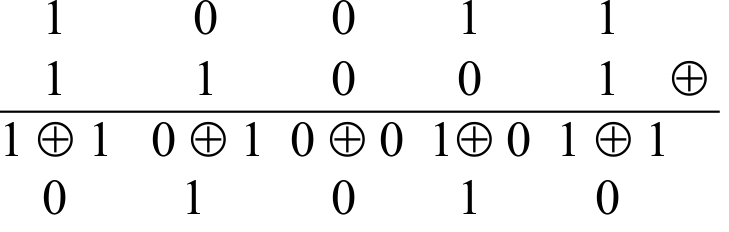
\includegraphics[width=79.80mm,height=63.85mm]{../../images/llm/page_011_img_01.png}%
\end{textblock*}

\end{document}
